\begin{subfigure}[b]{0.35\textwidth}
\centering
\raisebox{1\ht\strutbox}{
    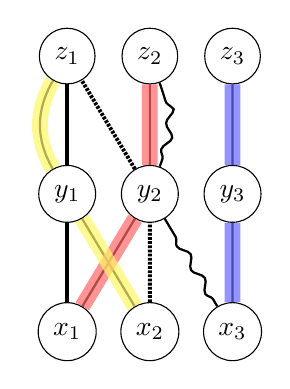
\begin{tikzpicture}[scale=0.7, transform shape = false, rotate=90]
        \pgfkeys{/nodeType/.style={circle, draw},
        /edgeType1/.style={solid, thick, line width=.5mm},
        /edgeType2/.style={solid, thick},
        /edgeType3/.style={thick, decorate, decoration={snake, amplitude=.5mm,pre=lineto,pre length=3pt,post=lineto,post length=3pt}},
        /edgeType4/.style={line width=2mm, draw opacity=0.7}} %highlights the edges of the solution
    
        \def\n{3}
        %n triples (x_i, y_j, z_k) of vertices
        \foreach \i in {1, ..., \n}{
            \node[/nodeType] (x\i) at (0, -1.5*\i) {$x_\i$}; 
            \node[/nodeType] (y\i) at (2.5, -1.5*\i) {$y_\i$}; 
            \node[/nodeType] (z\i) at (5, -1.5*\i) {$z_\i$};
        }
    
        %Edges
        \draw[/edgeType1] (x1) -- (y1) -- (z1);
        \draw[/edgeType2] (x1) -- (y2) -- (z2);
        \draw[/edgeType2] (x2) -- (y1) to[bend left=30] (z1);
        \draw[/edgeType1] [dotted, dash pattern=on 1pt off .5pt] (x2) -- (y2) -- (z1);
        \draw[/edgeType3] (x3) -- (y2);
        \draw[/edgeType3] (y2) to[bend right=20](z2);
        \draw[/edgeType2] (x3) -- (y3) -- (z3);
    
        %Solution
         \draw[/edgeType4] [red!60] (x1) -- (y2) -- (z2);
         \draw[/edgeType4] [yellow!60] (x2) -- (y1) to[bend left=30] (z1);
         \draw[/edgeType4] [blue!60] (x3) -- (y3) -- (z3);    
    \end{tikzpicture}
}
\caption{A \TDMT{} input instance}
\label{fig:sample3dm3}
\end{subfigure}
\quad
\begin{subfigure}[b]{0.58\textwidth}
\centering
\begin{tikzpicture}[scale=0.85, transform shape = false, rotate=90]
    \pgfkeys{/edgeType1/.style={solid, thick, line width=.5mm},
    /edgeType2/.style={solid, thick},
    /edgeType3/.style={thick, decorate, decoration={snake, amplitude=.5mm,pre=lineto,pre length=5pt,post=lineto,post length=5pt}},
    /edgeType4/.style={line width=2mm, green!60, draw opacity=0.7}} %highlights the edges of the solution

    %All vertices
    \node[circle, draw] (x1) at (-1.0, -1.25) {$x_1$};
    \node[circle, draw] (z1) at (4-0.5, -1.25) {$z_1$};
    \setVi{1}{0}{0}{2}
    \node[circle, draw] (x2) at (-1.0, -4.25) {$x_2$};
    \node[circle, draw] (z2) at (4-0.5, -4.25) {$z_2$};
    \setVi{2}{0}{-2.85}{3}
    \node[circle, draw] (x3) at (-1.0, -7.3) {$x_3$};
    \node[circle, draw] (z3) at (4-0.5, -7.3) {$z_3$};
    \setVi{3}{0}{-6.8}{1}

    %Edges
    \draw[/edgeType1] (x1) -- (y111);
    \draw[/edgeType1] (y112) -- (z1);
    \draw[/edgeType2] (y111) -- (y112);
    \draw[/edgeType2] (x2) -- (y121) -- (y122) -- (z1);
    \draw[/edgeType2] (x1) -- (y211) -- (y212) -- (z2);
    \draw[/edgeType1] [dotted, dash pattern=on 1pt off .5pt] (x2) -- (y221);
    \draw[/edgeType2] (y221) -- (y222);
    \draw[/edgeType1] [dotted, dash pattern=on 1pt off .5pt] (y222) -- (z1);
    \draw[/edgeType3] (x3) -- (y231);
    \draw[/edgeType2] (y231) -- (y232);
    \draw[/edgeType3] (y232) -- (z2);
    \draw[/edgeType2] (x3) -- (y311) -- (y312) -- (z3);

    %Solution
    \draw[/edgeType4] [red!60] (x1) -- (y211);
    \draw[/edgeType4] [red!60] (y212) -- (z2);
    \draw[/edgeType4] (y221) -- (y222);
    \draw[/edgeType4] (y231) -- (y232);
    \draw[/edgeType4] [yellow!60] (x2) -- (y121);
    \draw[/edgeType4] [yellow!60] (y122) -- (z1);
    \draw[/edgeType4] (y111) -- (y112);
    \draw[/edgeType4] [blue!60] (x3) -- (y311);
    \draw[/edgeType4] [blue!60] (y312) -- (z3);
\end{tikzpicture}
\caption{The corresponding \GRC{} instance}
\label{fig:sampleGRC}
\end{subfigure}